\documentclass[a4paper]{article}

\usepackage{inputenc}
\usepackage[british,UKenglish]{babel}
\usepackage{amsmath}
%\usepackage{titlesec}
\usepackage{color}
\usepackage{graphicx}
\usepackage{fancyref}
\usepackage{hyperref}
\usepackage{float}
\usepackage{scrextend}
\usepackage{setspace}
\usepackage{xargs}
\usepackage{multicol}
\usepackage{nameref}

\usepackage{sectsty}
\usepackage{multicol}
\usepackage{multirow}
\usepackage[procnames]{listings}
\usepackage{appendix}

\newcommand\tab[1][1cm]{\hspace*{#1}}
\hypersetup{colorlinks=true, linkcolor=black}
\interfootnotelinepenalty=10000

\newcommand{\cleancode}[1]{\begin{addmargin}[3em]{3em}\texttt{\textcolor{cleanOrange}{#1}}\end{addmargin}}
\newcommand{\cleanstyle}[1]{\text{\textcolor{cleanOrange}{\texttt{#1}}}}


\usepackage[colorinlistoftodos,prependcaption,textsize=footnotesize]{todonotes}
\newcommandx{\commred}[2][1=]{\textcolor{Red}
{\todo[linecolor=red,backgroundcolor=red!25,bordercolor=red,#1]{#2}}}
\newcommandx{\commblue}[2][1=]{\textcolor{Blue}
{\todo[linecolor=blue,backgroundcolor=blue!25,bordercolor=blue,#1]{#2}}}
\newcommandx{\commgreen}[2][1=]{\textcolor{OliveGreen}{\todo[linecolor=OliveGreen,backgroundcolor=OliveGreen!25,bordercolor=OliveGreen,#1]{#2}}}
\newcommandx{\commpurp}[2][1=]{\textcolor{Plum}{\todo[linecolor=Plum,backgroundcolor=Plum!25,bordercolor=Plum,#1]{#2}}}

\def\code#1{{\tt #1}}

\def\note#1{\noindent{\bf [Note: #1]}}

\makeatletter
%% The "\@seccntformat" command is an auxiliary command
%% (see pp. 26f. of 'The LaTeX Companion,' 2nd. ed.)
\def\@seccntformat#1{\@ifundefined{#1@cntformat}%
   {\csname the#1\endcsname\quad}  % default
   {\csname #1@cntformat\endcsname}% enable individual control
}
\let\oldappendix\appendix %% save current definition of \appendix
\renewcommand\appendix{%
    \oldappendix
    \newcommand{\section@cntformat}{\appendixname~\thesection\quad}
}
\makeatother


% "define" Scala
\usepackage[T1]{fontenc}  
\usepackage[scaled=0.82]{beramono}  
\usepackage{microtype} 

\sbox0{\small\ttfamily A}
\edef\mybasewidth{\the\wd0 }

\lstdefinelanguage{scala}{
  morekeywords={abstract,case,catch,class,def,%
    do,else,extends,false,final,finally,%
    for,if,implicit,import,match,mixin,%
    new,null,object,override,package,%
    private,protected,requires,return,sealed,%
    super,this,throw,trait,true,try,%
    type,val,var,while,with,yield},
  sensitive=true,
  morecomment=[l]{//},
  morecomment=[n]{/*}{*/},
  morestring=[b]",
  morestring=[b]',
  morestring=[b]"""
}

\usepackage{color}
\definecolor{dkgreen}{rgb}{0,0.6,0}
\definecolor{gray}{rgb}{0.5,0.5,0.5}
\definecolor{mauve}{rgb}{0.58,0,0.82}

% Default settings for code listings
\lstset{frame=tb,
  language=scala,
  aboveskip=3mm,
  belowskip=3mm,
  showstringspaces=false,
  columns=fixed, % basewidth=\mybasewidth,
  basicstyle={\small\ttfamily},
  numbers=none,
  numberstyle=\footnotesize\color{gray},
  % identifierstyle=\color{red},
  keywordstyle=\color{blue},
  commentstyle=\color{dkgreen},
  stringstyle=\color{mauve},
  frame=single,
  breaklines=true,
  breakatwhitespace=true,
  procnamekeys={def, val, var, class, trait, object, extends},
  procnamestyle=\ttfamily\color{red},
  tabsize=2
}

\lstnewenvironment{scala}[1][]
{\lstset{language=scala,#1}}
{}
\lstnewenvironment{cpp}[1][]
{\lstset{language=C++,#1}}
{}
\lstnewenvironment{bash}[1][]
{\lstset{language=bash,#1}}
{}
\lstnewenvironment{verilog}[1][]
{\lstset{language=verilog,#1}}
{}



\lstset{frame=,basicstyle={\footnotesize\ttfamily}}



\graphicspath{ {images/} }
\usepackage{ctex}
\usepackage{verbatim}
\usepackage{geometry}
\usepackage{amsmath}
\usepackage{pifont}%\ding{192} \ding{172}
\usepackage{tikz}
\usepackage{float}
\usepackage{booktabs}
\usepackage{bm}
\usepackage{siunitx}
\usepackage{enumerate}
\usepackage{cite}
%\usepackage{graphicx}
%\geometry{a4paper, scale=0.72}
\geometry{a4paper,left=2.5cm,right=2.5cm,top=2.5cm,bottom=2.5cm}
%%%%%%%%%%%%%%%%%%%%%%%%%%%%%%%%%%%%%%%% BEGIN DOC %%%%%%%%%%%%%%%%%%%%%%%%%%%%%%%%%%%%%%%%

\begin{document}
\renewcommand{\contentsname}{目\ 录}
\renewcommand{\appendixname}{附录}
\renewcommand{\appendixpagename}{附录}
\renewcommand{\refname}{参考文献} 
\renewcommand{\figurename}{图}
\renewcommand{\tablename}{表}
\renewcommand{\today}{\number\year 年 \number\month 月 \number\day 日}
\newcommand{\refeq}[1]{\textbf{Eq.(\ref{#1})}}
\newcommand*{\circled}[1]{\lower.7ex\hbox{\tikz\draw (0pt, 0pt)%
    circle (.5em) node {\makebox[1em][c]{\small #1}};}}
    
\title{{\Huge 近代物理实验报告{\large\linebreak\\}}{\Large 实验5-4:\ 扫描隧穿显微镜\linebreak\linebreak}}
%please write your name, Student #, and Class # in Authors, student ID, and class # respectively
\author{\\姓\ 名:付\ 大\ 为\\
学\ 号: 1800011105\\
邮\ 箱: \url{fudw@pku.edu.cn}\\
%班\ 号: xxxxx\\\\
近代物理实验 (II)\\
(2022,春季学期)\\\\
北京大学\\
物理学院\\
2018级1班}
\date{\today}
\maketitle
\newpage

%%%%%%%%%%%%%%%%%%%%%%%%%%%%%%%%%%%%%%%% ABSTRACT %%%%%%%%%%%%%%%%%%%%%%%%%%%%%%%%%%%%%%%%
\begin{center}
{\Large\bf{摘\ 要\\}}
\end{center}

本实验使用扫描隧穿显微镜(Scanning tunneling microscope, STM)获得了样品表面的原子分辨像,从而直观地验证量子隧穿效应;同时,总结了隧穿电流的变化规律,并在此基础上探讨了隧穿显微技术的应用。

实验中观察的样品为结构已知的高定向热解石墨(Highly oriented pyrolytic graphite, HOGP);本实验通过比较STM所成图像与样品实际结构,粗略地校准了STM的探针控制系统,从而使其能较为精确地获得结构未知样品的原子分辨像。
\\\\
{\bf{关键词}:}\ 热对流,非线性斑图,耗散

%%%%%%%%%%%%%%%%%%%%%%%%%%%%%%%%%%%%%%%% CONTENT %%%%%%%%%%%%%%%%%%%%%%%%%%%%%%%%%%%%%%%%
\newpage
\begin{center}
\tableofcontents\label{c}
\end{center}
\newpage

%%%%%%%%%%%%%%%%%%%%%%%%%%%%%%%%%%%%%%%% Introduction %%%%%%%%%%%%%%%%%%%%%%%%%%%%%%%%%%%%%%%%
\section{引言} \label{overview}%------------------------------
在一定条件下,微观粒子能够穿入或穿越高于其总能量的势垒;这一极端非经典的现象称为隧穿效应(Quantum tunneling)。
	
早在1901年,Robert Francis Earhart在研究气体放电时发现了异常的电导,这可能是隧穿效应的首个实验迹象。在此后的20余年间,实验中多次观测到隧穿电流,但并没有成熟的理论解释;事实上,由于观测到的隧穿电流十分微弱(在 \SI{10}{\pA} 量级),这一效应并没有得到充分的重视\supercite{mohsen2003quantum}。
	
1926年,薛定谔发表了波动方程,严谨的量子力学体系得以建立;在此基础上,1927年洪德(Friedrich Hund)首次从理论上发现了隧穿效应,他和伽莫夫(George Gamow)等人将其应用于原子核衰变的研究中;但当时人们并没有意识到,这一现象不仅局限于核物理范畴,还能有可直接观测的效应\supercite{mohsen2003quantum}。
	
隧穿在量子体系中的普遍存在是波恩(Max Born)首先提出的;在随后关于半导体的研究中,这一观点被充分证实,此后隧穿及其理论解释才被广泛地接受\supercite{mohsen2003quantum}。
	
1981年,IBM苏黎世实验室的格尔德·宾宁(G.~Binging)和海因里希·罗雷尔(H.~Rohrer)首次成功利用隧穿效应获得了原子分辨像,发明了第一台扫描隧穿显微镜(STM, scanning tunneling microscope)。STM的工作强烈地依赖于精确到 \si{\angstrom} 量级的位置控制,这通过对压电陶瓷加压得以实现。事实上,完全类似的想法曾由R.~Young等人在1970年代初期提出, 但由于技术上的限制,他们未能得到出色的结果。1986年,STM获得诺贝尔物理学奖。
	
本次实验中,我们力图采用完全类似的方法,重现宾宁和罗雷尔的实验;通过观测已知的材料——高定向热解石墨(HOPG, Highly oriented pyrolytic graphite),验证这一技术的有效性。此外,我们将考察压电材料在此实验中所起的关键作用,并检验本实验采用的陶瓷之压电特性。由于水平面上的精准定位对成像质量(防止畸变)尤为重要,我们将仅考察控制$x,y$位置的压电陶瓷,以此粗略地校准定位系统,为精准测定创造条件。

%%%%%%%%%%%%%%%%%%%%%%%%%%%%%%%%%%%%%%%% Theory %%%%%%%%%%%%%%%%%%%%%%%%%%%%%%%%%%%%%%%%
\newpage
\section{理论} \label{theory}%------------------------------
简单起见,考察一维定态薛定谔方程:
\begin{equation}
	- \frac{\hbar^2}{2m}\psi(x) + [\big{V(x) - E}]\psi(x) = 0
\end{equation}
以此描述针尖与样品之间的电子流。首先,对于不存在势垒的情况(\textit{可以想象针尖与样品表面以导电介质连通}),此时在一定的偏压下,稳恒电子流可由平面波函数描述:
\begin{equation}
	\psi(x) \sim e^{ikx},\quad
	k = \frac{p}{\hbar} = \frac{\sqrt{2mE}}{\hbar}
\end{equation}


若存在势垒,设其高度为$\phi$, 而针尖位于$x = 0$处,样品表面位于$x = s$处,则$V(x)$的分布可以粗略地表示为:
\begin{equation}
	V(x) = \Bigg\lbrace\,
	\begin{aligned}
		\phi, \quad& 0 < x < s,\\
		0, \quad& x < 0 \ \textrm{or}\  x > s, 
	\end{aligned}
\end{equation}
如\autoref{fig:Tunnel1D} 所示,其中入射波、反射波、透射波均采用平面波近似:
\begin{equation}
	\textit{入射:} e^{ikx},\quad
	\textit{反射:} R\,e^{-ikx},\quad
	\textit{透射:} T\,e^{ikx},
\end{equation}

求解薛定谔方程,我们发现,$0 < x < s$区域内的波函数并不为0, 而是具有指数衰减的形式:
\begin{gather}
	\psi(x) \propto e^{-\kappa x},\quad 0 < x < s,\\
	\kappa = \frac{\sqrt{2m(\phi - E)}}{\hbar}
		\sim \frac{\sqrt{2m\phi}}{\hbar}
\end{gather}
这里采用了近似处理,假定势垒高度$\phi \gg E$. 进一步,由于电流$I$与电子透射率线性相关,求解得到:
\begin{equation}
	\frac{I}{I_0} = \abs{T}^2
	\sim \frac{16E}{\phi} e^{-2\kappa s},\quad
	\kappa \sim \frac{\sqrt{2m\phi}}{\hbar}
\end{equation}
同样采用了近似条件$\phi \gg E$, 其中$I_0$为势垒为0时的电流大小。

综上,我们得到了隧穿电流的估计式:
\begin{equation}
	I \sim B\,e^{-2\kappa s},\quad
	\kappa \sim \frac{\sqrt{2m\phi}}{\hbar},\quad
	B \sim I_0 \frac{16E}{\phi}
	\label{eq:tunnelEq}
\end{equation}
针尖与样品之间所加的偏压$V_\textup{b}$越大,相应的$I_0, E$越大,隧穿电流越大;同时,势垒宽度$s$越大,隧穿电流越小,且为指数衰减。在控制真空度一定的情形下,可以假定势垒高度$\phi$基本恒定。

工作状态下,本实验中的STM针尖与样品间距$s \sim \SI{1}{\nm} = \SI{10}{\angstrom}$, 电流改变一个量级对应的$\var{s} \sim \SI{0.1}{\nm} = \SI{1}{\angstrom}$, 正是原子间距的尺度。
这自然导致了STM的高分辨率,同时也对装置的机械稳定性提出了很高的要求。
	
此外,这也表明隧穿电流局域在针尖和样品原子间极端细长的范围内,此区域内上述一维模型基本成立;针尖附近隧穿电流的实际分布如所示。
%%%%%%%%%%%%%%%%%%%%%%%%%%%%%%%%%%%%%%%% Experiment %%%%%%%%%%%%%%%%%%%%%%%%%%%%%%%%%%%%%%%%
\newpage
\section{实验} \label{experiment}%------------------------------
\subsection{实验仪器}\label{sub:instruments}
\begin{itemize}
\item{\textbf{减震系统}}

本实验所使用的STM系统配置的是有效但很廉价的多级减震系统
\begin{enumerate}[(1)]
    \item 用于隔离低频振动的挂在系统上的四根长的弹簧.
    \item 在STM系统的底盘上加氟橡胶条使系统的性能进一步完善.
\end{enumerate}
\item{\textbf{粗逼近}}

粗逼近的目标是把样品移动到扫描架工作的范围内,并且要求它在不工作时要尽可能稳定地停在它的位置上,以减小振动的影响.
\item{\textbf{扫描架}}

本仪器的扫描架由两对陶瓷杆和一根陶瓷管支撑着的牢固结构组成.两对陶瓷杆的材料、压电系数和长度是一样的
\item{\textbf{STM电子学控制单元}}

STM由一台PC机和电子学单元控制,它们之间通过一8825接口卡来连接,电子学分为工作电源和隧穿电流反馈控制与信号采集两大部分.

\end{itemize}

%------------------------------------------------------------
\subsection{简要实验步骤}\label{sub:ExperimentalSteps}
分为以下几个步骤:\\\\
\circled{1}熟悉控制和处理程序\\\\
\circled{2}得到石墨的原子分辨像\\\\
\circled{3}观察金膜表面\\\\
\circled{4}标定x、y陶瓷的压电系数\\\\

%%%%%%%%%%%%%%%%%%%%%%%%%%%%%%%%%%%%%%%% Results & Discussions %%%%%%%%%%%%%%%%%%%%%%%%%%%%%%%%%%%%%%%%
\newpage
\section{结果及讨论}
%------------------------------------------------------------
\subsection{大范围扫描}\label{sub:1}
开始时设置偏压$V_b=\SI{1000}{m\volt}$,$V_z=\SI{200}{\volt}$,扫描时间$T=\SI{2000}{m\s}$,大范围扫描结果如下\textbf{图\ref{result:fig1}}所示 
\begin{figure}[H]
 \centering
 \caption{$V_b=\SI{1000}{m\volt}$,$V_z=\SI{200}{\volt}$,$T=\SI{2000}{m\s}$}
 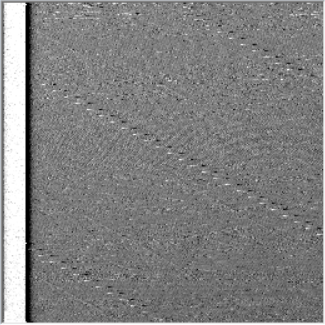
\includegraphics[height=10cm, width=10cm]{images/200V-1000mV-2000ms.png}
 \label{result:fig1}
\end{figure}
此时还没有出现原子分辨迹象.
到$V_b=\SI{1000}{m\volt}$,$V_z=\SI{50}{\volt}$,$T=\SI{800}{m\s}$时候开始出现原子分辨迹象如下\textbf{图\ref{result:fig2}}所示
\begin{figure}[H]
 \centering
 \caption{$V_b=\SI{1000}{m\volt}$,$V_z=\SI{50}{\volt}$,$T=\SI{800}{m\s}$}
 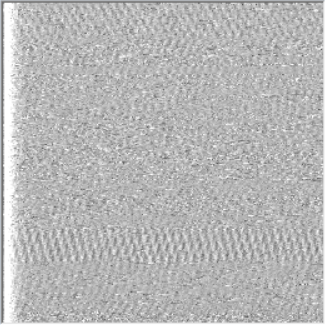
\includegraphics[height=10cm, width=10cm]{images/50V-1000mV-800ms.png}
 \label{result:fig2}
\end{figure}
到$V_b=\SI{1000}{m\volt}$,$V_z=\SI{10}{\volt}$,$T=\SI{400}{m\s}$时进一步增强到如下\textbf{图\ref{result:fig3}}所示
\begin{figure}[H]
 \centering
 \caption{$V_b=\SI{1000}{m\volt}$,$V_z=\SI{10}{\volt}$,$T=\SI{400}{m\s}$}
 
\includegraphics[height=10cm, width=10cm]{images/10V-1000mV-400ms.png}
 \label{result:fig3}
\end{figure}
此时已经有接近清晰原子分辨像出现,接着分别在$V_z=\SI{4}{\volt}$和$V_z=\SI{2}{\volt}$时改变扫描时间寻找最清晰成像
%------------------------------------------------------------
\subsection{在$V_z=\SI{4}{\volt}$时寻找最清晰原子成像}\label{sub:2}
$V_b=\SI{1000}{m\volt}$,$V_z=\SI{4}{\volt}$,$T=\SI{400}{m\s}$时成像如下\textbf{图\ref{result:fig4}}所示
\begin{figure}[H]
 \centering
 \caption{$V_b=\SI{1000}{m\volt}$,$V_z=\SI{4}{\volt}$,$T=\SI{400}{m\s}$}
 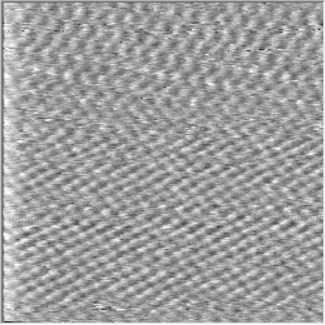
\includegraphics[height=10cm, width=10cm]{images/4v-1000mv-400ms.png}
 \label{result:fig4}
\end{figure}
$V_b=\SI{1000}{m\volt}$,$V_z=\SI{4}{\volt}$,$T=\SI{300}{m\s}$时成像如下\textbf{图\ref{result:fig5}}所示
\begin{figure}[H]
 \centering
 \caption{$V_b=\SI{1000}{m\volt}$,$V_z=\SI{4}{\volt}$,$T=\SI{300}{m\s}$}
 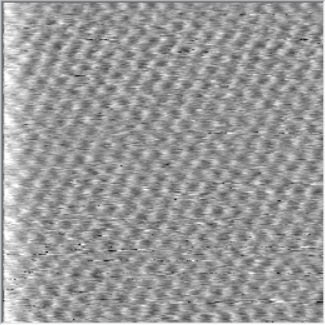
\includegraphics[height=10cm, width=10cm]{images/4V-1000mV-300ms.png}
 \label{result:fig5}
\end{figure}
$V_b=\SI{1000}{m\volt}$,$V_z=\SI{4}{\volt}$,$T=\SI{200}{m\s}$时成像如下\textbf{图\ref{result:fig6}}所示结果
\begin{figure}[H]
 \centering
 \caption{$V_b=\SI{1000}{m\volt}$,$V_z=\SI{4}{\volt}$,$T=\SI{200}{m\s}$}
 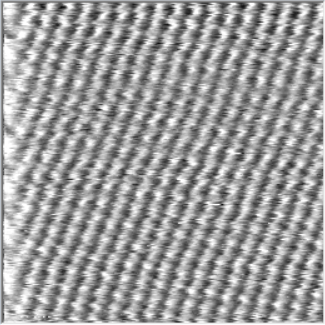
\includegraphics[height=10cm, width=10cm]{images/4v-1000mv-200ms.png}
 \label{result:fig6}
\end{figure}
此时已接近$V_z=\SI{4}{\volt}$最清晰原子成像
%------------------------------------------------------------
\subsection{在$V_z=\SI{2}{\volt}$时寻找最清晰原子成像}\label{sub:3}
$V_b=\SI{1000}{m\volt}$,$V_z=\SI{2}{\volt}$,$T=\SI{300}{m\s}$时成像如下\textbf{图\ref{result:fig7}}所示
\begin{figure}[H]
 \centering
 \caption{$V_b=\SI{1000}{m\volt}$,$V_z=\SI{2}{\volt}$,$T=\SI{300}{m\s}$}
 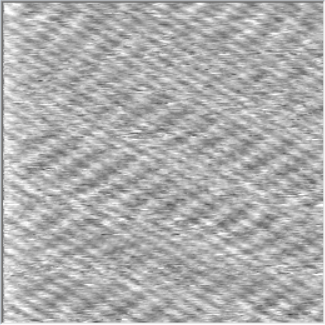
\includegraphics[height=9cm, width=9cm]{images/2V-1000mV-300ms.png}
 \label{result:fig7}
\end{figure}
$V_b=\SI{300}{m\volt}$,$V_z=\SI{2}{\volt}$,$T=\SI{500}{m\s}$时成像如下\textbf{图\ref{result:fig8}}所示
\begin{figure}[H]
 \centering
 \caption{$V_b=\SI{300}{m\volt}$,$V_z=\SI{2}{\volt}$,$T=\SI{500}{m\s}$}
 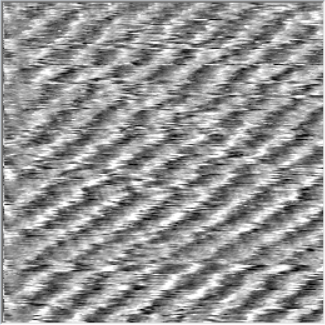
\includegraphics[height=10cm, width=10cm]{images/2v-300mv-500ms.png}
 \label{result:fig8}
\end{figure}
$V_b=\SI{300}{m\volt}$,$V_z=\SI{2}{\volt}$,$T=\SI{60}{m\s}$时成像如下\textbf{图\ref{result:fig9}}所示
\begin{figure}[H]
 \centering
 \caption{$V_b=\SI{300}{m\volt}$,$V_z=\SI{2}{\volt}$,$T=\SI{60}{m\s}$}
 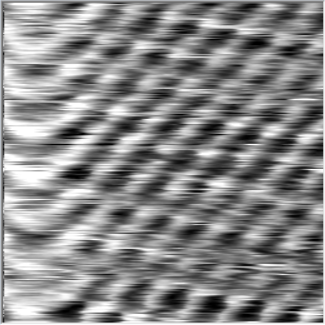
\includegraphics[height=10cm, width=10cm]{images/2v-300mv-60ms.png}
 \label{result:fig9}
\end{figure}
此时可以看到清晰的原子图样.
%add more subsections for other block
%%%%%%%%%%%%%%%%%%%%%%%%%%%%%%%%%%%%%%%% Conclusion %%%%%%%%%%%%%%%%%%%%%%%%%%%%%%%%%%%%%%%%
\section{结论}\label{conclusions}
本实验对高定向热解石墨(HOPG)样品表面进行了STM扫描和测量,观察并得到了其原子级分辨像,并对像的结构进行了简单的解释。
	
本实验所获得的原子分辨像是对隧穿效应乃至原子论的最强有力验证。这一技术突出了精准控制与精确测量的重要性,这也是实现该技术的主要困难;同时,STM的直观性也揭示了其巨大的潜能,预示着扫描探针显微技术将在科学研究和纳米加工技 术中发挥出越来越大的作用。

%%%%%%%%%%%%%%%%%%%%%%%%%%%%%%%%%%%%%%%% Questions %%%%%%%%%%%%%%%%%%%%%%%%%%%%%%%%%%%%%%%%
\begin{comment}
\section{实验报告思考题}\label{questions}
\subsection{在$a=23.0mm$、$b=10.0mm$的矩形波导管中能不能传播$\lambda=2cm$、$3cm$和$5cm$的微波?各能传播哪些波型?}\label{sub:question1}
答:根据
\begin{equation}
    \lambda_c=\frac{2}{\sqrt{(m/a)^2+(n/b)^2}}
\end{equation}
我们可以算出可传播的最大波长为$\lambda_{max}=18.3mm$,显然不能传播$\lambda=2cm$、$3cm$和$5cm$的微波,可传输波长在$\lambda_{max}=18.3mm$以下,满足$\lambda_c=\frac{2}{\sqrt{(m/a)^2+(n/b)^2}}$的波长的波型\\

\end{comment}

%%%%%%%%%%%%%%%%%%%%%%%%%%%%%%%%%%%%%%%% Acknowledgements %%%%%%%%%%%%%%%%%%%%%%%%%%%%%%%%%%%%%%%%

\section{致谢}\label{acknowledgments}
感谢老师在实验中的的悉心指导.

\begin{comment}
%%%%%%%%%%%%%%%%%%%%%%%%%%%%%%%%%%%%%%%% Appendix %%%%%%%%%%%%%%%%%%%%%%%%%%%%%%%%%%%%%%%%
\appendix
\section{代码}\label{sub:app.code}
请在附录\ref{sub:app.code}中添加代码。请使用如下Scala的语法高亮描述方法。
\begin{scala}
class TopIO extends Bundle() {
	val boot = Input(Bool()) 
// imem and dmem interface for Tests
	val test_im_wr		= Input(Bool())
	val test_im_rd 		= Input(Bool())
	val test_im_addr 	= Input(UInt(32.W))
	val test_im_in 		= Input(UInt(32.W))
	val test_im_out 	= Output(UInt(32.W))

	val test_dm_wr		= Input(Bool())
	val test_dm_rd 		= Input(Bool())
	val test_dm_addr 	= Input(UInt(32.W))
	val test_dm_in 		= Input(UInt(32.W))
	val test_dm_out 	= Output(UInt(32.W))

	val valid			= Output(Bool())
}
class Top extends Module() {
	val io 		= IO(new TopIO())//in chisel3, io must be wrapped in IO(...) 
	//...
	when (io.boot & io.test_im_wr){
		imm(io.test_im_addr) := io.test_im_in
		} .elsewhen (io.boot & io.test_dm_wr){
		// please finish it
		} //...
}
\end{scala}
\newpage
\end{comment}
%%%%%%%%%%%%%%%%%%%%%%%%%%%%%%%%%%%%%%%% REFERENCE %%%%%%%%%%%%%%%%%%%%%%%%%%%%%%%%%%%%%%%%
\bibliographystyle{unsrt}
\bibliography{Ref}
\nocite{*}

\end{document}

